\chapter{Resultados e Discussões}
\label{chap:resultados}

Após a construção do filtro tipo prensa, foram realizados inúmeros
procedimentos, a partir de diferentes soluções com partículas indesejadas a fim
de verificar a funcionalidade do filtro.

Os resultados obtidos foram satisfatórios, pois em todos os procedimentos
realizados foi possível a obtenção de uma solução com menor teor de partículas
aparentemente.

Os procedimentos realizados seguem descritos abaixo.

\section{Primeiro procedimento}
\label{sec:proc1}

\textbf{Contaminante:} partículas aleatórias de terra.

\textbf{Solvente:} água.

De forma simplista, foram realizados três testes preliminares com solução
contendo o contaminante sem granulometria conhecida,a fim de verificar
a funcionalidade do sistema construído, tal como sua vedação.

Os testes mostraram pontos de vazamentos na estrutura de madeira e também
pressão insuficiente na alimentação, que não permitia que a solução atingisse
todas as membranas filtrantes. Com isso, o projeto sofreu as seguintes
alterações:

\begin{itemize}
\item Utilização de uma garrafa maior que alimenta o fluido ao sistema,
  permitindo bombeamento manual mais intenso e fácil,
\item Utilização de silicone para vedar os pontos de vazamento da solução.
\end{itemize}

A solução filtrada obtida continha pequenas partículas e apresentava coloração
marrom clara.


\section{Segundo procedimento}
\label{sec:proc2}

\textbf{Contaminante:} mistura contendo as partículas apresentadas na Tabela
\ref{granulometria2}.

\textbf{Solvente:} água.

% \cite{milho}
% \cite{MASSON1984}
% \cite{alessi2009caracterizaccao}
% \cite{guarienti1993qualidade}

\begin{table}[H]
\centering
\caption{Granulometria das partículas utilizadas no segundo procedimento. Dados
  retirados de \citeay{alessi2009caracterizaccao},
  \citeay{guarienti1993qualidade}, \citeay{milho} e \citeay{MASSON1984}.}
\label{granulometria2}
\begin{tabular}{@{}lr@{}}
\toprule
\multicolumn{1}{c}{\textbf{Partícula}} & \multicolumn{1}{c}{\textbf{Diâmetro aproximado (\si{mm})}} \\ \midrule
Canjiquinha      & 1,18 \\
Fubá             & 0,34 \\
Pó de café       & 0,59 \\
Trigo para quibe & 1,05 \\  \bottomrule
\end{tabular}
\end{table}

Por conter partículas que não se dissolveram adequadamente devido a seus grandes
diâmetros como a canjiquinha e o trigo para quibe, houve aglomeraração nos tubos
de alimentação do filtro, formando tortas.

A formação de tortas na entrada do filtro propiciou uma pré filtração das
partículas menores, gerando uma maior eficiência do filtro, como pode-se
observar na Figura \ref{fig:proc2}, onde todas as membranas do filtro
contribuíram para a filtração, produzindo um produto com menor teor de
partículas.

\begin{figure}[H]
  \centering
  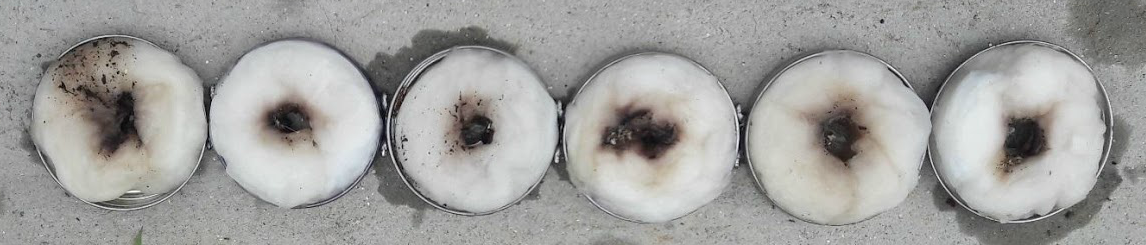
\includegraphics[width=0.9\textwidth]{figuras/proc2.png}
  \caption{Membranas filtrantes após a realização do segundo
    procedimento.\label{fig:proc2}}
\end{figure}

A solução final obtida após o processo apresentou-se límpida, transparente e sem
partículas aparentes.


\section{Terceiro procedimento}
\label{sec:proc3}

\textbf{Contaminante:} mistura contendo pó de café e fubá. O
diâmetro aproximado dessas partículas pode ser observado na Tabela
\ref{granulometria2}.

\textbf{Solvente:} água.

Com a utilização de partículas de menor diâmetro não foi possível obter um
filtrado mais límpido do que o obtido no segundo procedimento, pois devido a
pequena dimensão das partículas as membranas filtrantes não conseguiram retê-las
com tanta eficiência.

Foi possível observar uma maior retenção de partículas de pó de café nas
primeiras membranas do filtro, concentradas em seu centro. Neste procedimento,
as partículas de fubá não ficaram visíveis nas membranas.

A solução obtida após a realização do procedimento apresentou resquícios de
partículas e coloração amarelada. Portanto, pode-se dizer que a formação de
torta no procedimento anterior favoreceu a filtração do sistema e, sem a
formação de torta, percebe-se que as membranas filtrantes (algodões) não são tão
eficientes para a retenção de partículas de menores diâmetros.


% \begin{table}[H]
% \centering
% \caption{Granulometria das partículas utilizadas no terceiro procedimento.}
% \label{granulometria3}
% \begin{tabular}{@{}lr@{}}
% \toprule
% \multicolumn{1}{c}{\textbf{Partícula}} & \multicolumn{1}{c}{\textbf{Diâmetro aproximado (\si{mm})}} \\ \midrule
% fubá                       & 0,34                                                 \\
% Pó de café                       & 0,59                                                 \\ \bottomrule
% \end{tabular}
% \end{table}

%%% Local Variables:
%%% mode: latex
%%% TeX-master: "../main_archive"
%%% End:
